\input{javapractstyle}
\author{Pieter~van~den~Hombergh}
\title{Statemachines, find the differences}
\begin{document}

\section*{Guards and choices revisited}
\begin{figure}\centering
  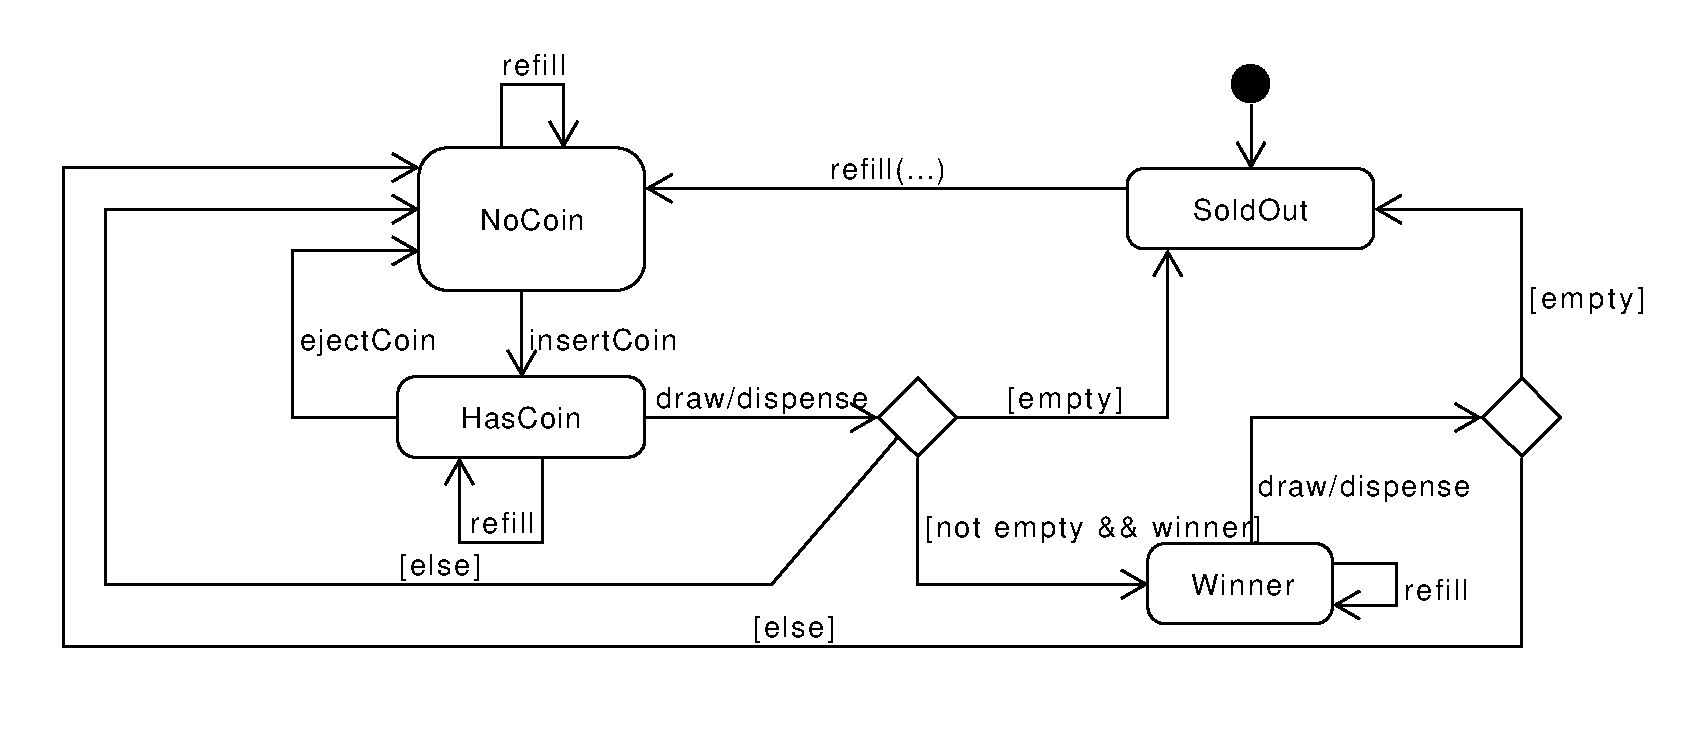
\includegraphics[width=.9\linewidth]{figures/statemachine}
  \caption{\label{d1}State diagram v1.0, using choices and
    dynamic evaluation}
\end{figure}

\begin{figure}\centering
  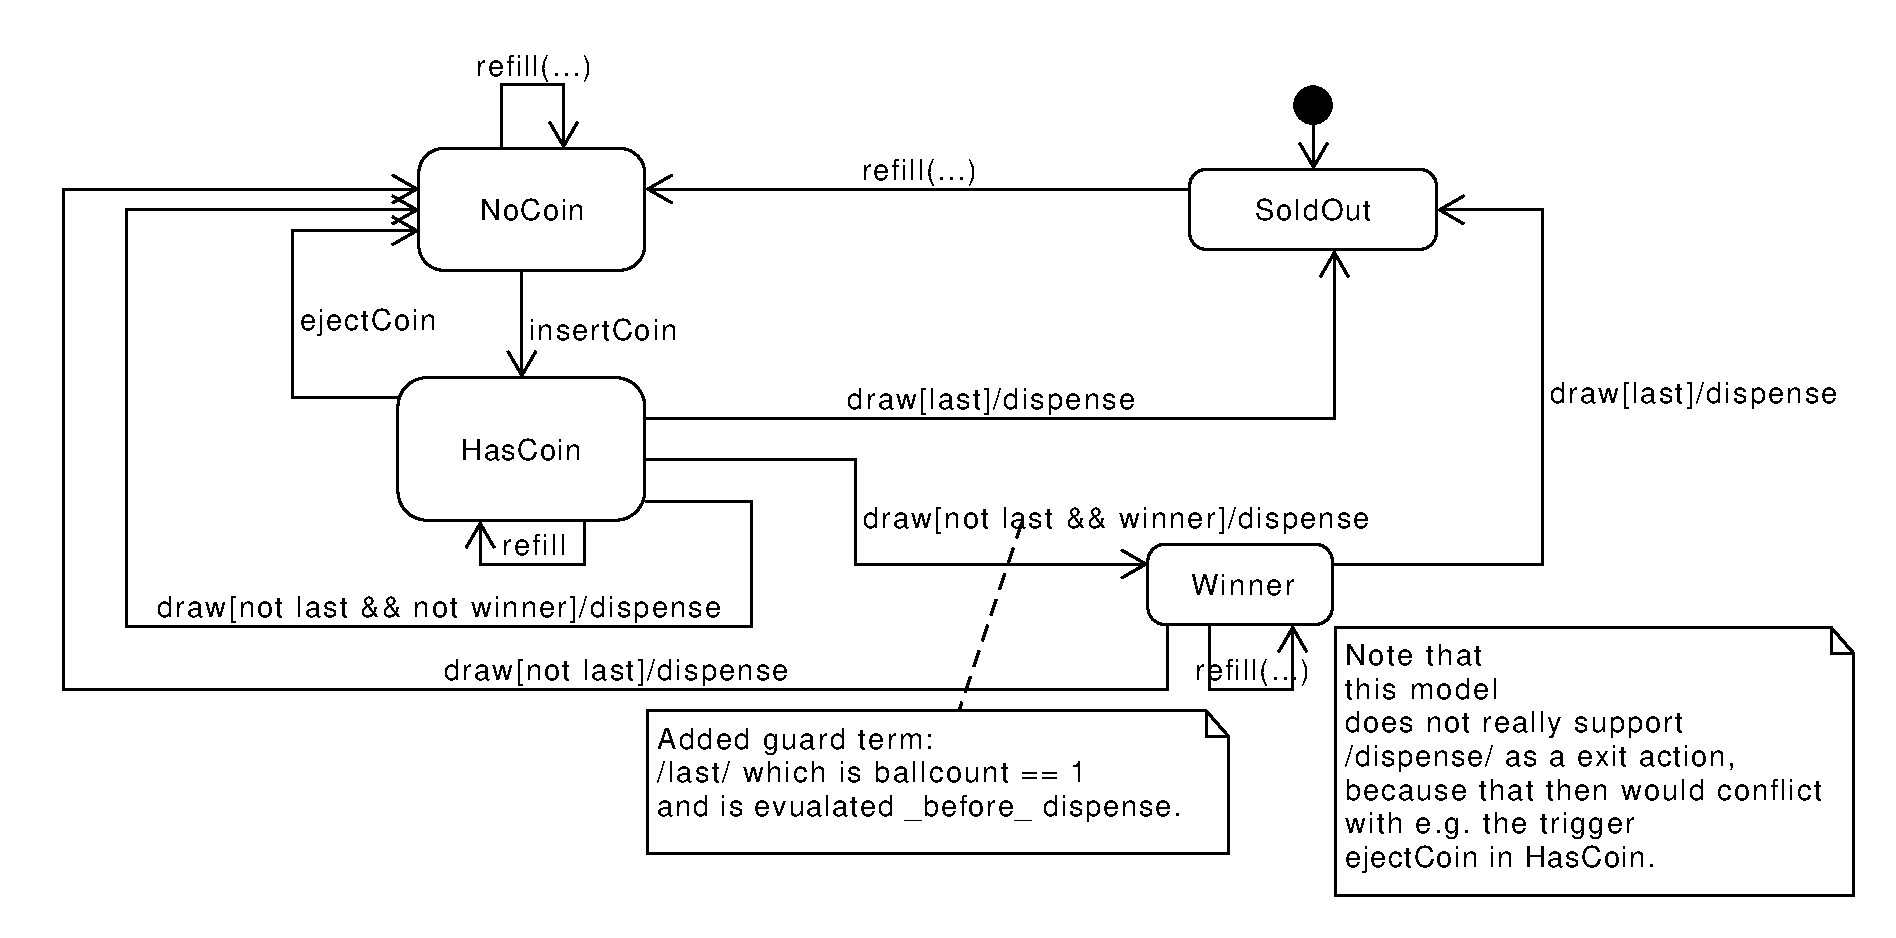
\includegraphics[width=.9\linewidth]{figures/statemachine3}
  \caption{\label{d2}Only using guards}
\end{figure}

Diagram~\ref{d1} is an allowed form in UML, using choice pseudo states that
always resolve ([else] or default).
\
\begin{itemize}
\item Dynamic evaluation is allowed on a transition and may use the results
  of actions (dispense in the example) on that transition.
\item This approach MUST always have one guard active OR should have a
  default a.k.a. else. Rationale: you started the transition and you
  must have a valid way out. NOT fulfilling this constraint leads to an
  ill formed state diagram.
\end{itemize}


Diagram~\ref{d2} has a more strict interpretation: Use guards on transitions.

\begin{itemize}
\item This approach disallows what is allowed in diagram~\ref{d1}: dynamic evaluation
and then make up your mind (in the example: dispense and then look at
the empty condition). Diagram MUST evaluate its guard first, which
needs an extra condition to be considered: \textbf{last}. Rationale:
you can not partly start a transition and then retract, so everything
must be evaluated before you can consider which of the guarded
variants you may choose. 
\item This solution DOES support all guards to be false, in which case the
transition is NOT considered.
\end{itemize}

\vspace{\baselineskip}
Bottom line: The approaches are both valid, non contradictory and
complementing each other.

Venlo 2016-05-17.



\end{document}
